
%% bare_jrnl.tex
%% V1.4b
%% 2015/08/26
%% by Michael Shell
%% see http://www.michaelshell.org/
%% for current contact information.
%%
%% This is a skeleton file demonstrating the use of IEEEtran.cls
%% (requires IEEEtran.cls version 1.8b or later) with an IEEE
%% journal paper.
%%
%% Support sites:
%% http://www.michaelshell.org/tex/ieeetran/
%% http://www.ctan.org/pkg/ieeetran
%% and
%% http://www.ieee.org/

%%*************************************************************************
%% Legal Notice:
%% This code is offered as-is without any warranty either expressed or
%% implied; without even the implied warranty of MERCHANTABILITY or
%% FITNESS FOR A PARTICULAR PURPOSE! 
%% User assumes all risk.
%% In no event shall the IEEE or any contributor to this code be liable for
%% any damages or losses, including, but not limited to, incidental,
%% consequential, or any other damages, resulting from the use or misuse
%% of any information contained here.
%%
%% All comments are the opinions of their respective authors and are not
%% necessarily endorsed by the IEEE.
%%
%% This work is distributed under the LaTeX Project Public License (LPPL)
%% ( http://www.latex-project.org/ ) version 1.3, and may be freely used,
%% distributed and modified. A copy of the LPPL, version 1.3, is included
%% in the base LaTeX documentation of all distributions of LaTeX released
%% 2003/12/01 or later.
%% Retain all contribution notices and credits.
%% ** Modified files should be clearly indicated as such, including  **
%% ** renaming them and changing author support contact information. **
%%*************************************************************************


% *** Authors should verify (and, if needed, correct) their LaTeX system  ***
% *** with the testflow diagnostic prior to trusting their LaTeX platform ***
% *** with production work. The IEEE's font choices and paper sizes can   ***
% *** trigger bugs that do not appear when using other class files.       ***                          ***
% The testflow support page is at:
% http://www.michaelshell.org/tex/testflow/



\documentclass[journal,12pt,twocolumn]{IEEEtran}

%draftclsnofoot
%
% If IEEEtran.cls has not been installed into the LaTeX system files,
% manually specify the path to it like:
% \documentclass[journal]{../sty/IEEEtran}





% Some very useful LaTeX packages include:
% (uncomment the ones you want to load)


% *** MISC UTILITY PACKAGES ***
%
%\usepackage{ifpdf}
% Heiko Oberdiek's ifpdf.sty is very useful if you need conditional
% compilation based on whether the output is pdf or dvi.
% usage:
% \ifpdf
%   % pdf code
% \else
%   % dvi code
% \fi
% The latest version of ifpdf.sty can be obtained from:
% http://www.ctan.org/pkg/ifpdf
% Also, note that IEEEtran.cls V1.7 and later provides a builtin
% \ifCLASSINFOpdf conditional that works the same way.
% When switching from latex to pdflatex and vice-versa, the compiler may
% have to be run twice to clear warning/error messages.






% *** CITATION PACKAGES ***
%
\usepackage{cite}
% cite.sty was written by Donald Arseneau
% V1.6 and later of IEEEtran pre-defines the format of the cite.sty package
% \cite{} output to follow that of the IEEE. Loading the cite package will
% result in citation numbers being automatically sorted and properly
% "compressed/ranged". e.g., [1], [9], [2], [7], [5], [6] without using
% cite.sty will become [1], [2], [5]--[7], [9] using cite.sty. cite.sty's
% \cite will automatically add leading space, if needed. Use cite.sty's
% noadjust option (cite.sty V3.8 and later) if you want to turn this off
% such as if a citation ever needs to be enclosed in parenthesis.
% cite.sty is already installed on most LaTeX systems. Be sure and use
% version 5.0 (2009-03-20) and later if using hyperref.sty.
% The latest version can be obtained at:
% http://www.ctan.org/pkg/cite
% The documentation is contained in the cite.sty file itself.



\usepackage{upgreek}


% *** GRAPHICS RELATED PACKAGES ***
%
\ifCLASSINFOpdf
  \usepackage[pdftex]{graphicx}
  % declare the path(s) where your graphic files are
  % \graphicspath{{../pdf/}{../jpeg/}}
  % and their extensions so you won't have to specify these with
  % every instance of \includegraphics
   \DeclareGraphicsExtensions{.pdf,.jpeg,.png}
\else
  % or other class option (dvipsone, dvipdf, if not using dvips). graphicx
  % will default to the driver specified in the system graphics.cfg if no
  % driver is specified.
  % \usepackage[dvips]{graphicx}
  % declare the path(s) where your graphic files are
  % \graphicspath{{../eps/}}
  % and their extensions so you won't have to specify these with
  % every instance of \includegraphics
  % \DeclareGraphicsExtensions{.eps}
\fi
% graphicx was written by David Carlisle and Sebastian Rahtz. It is
% required if you want graphics, photos, etc. graphicx.sty is already
% installed on most LaTeX systems. The latest version and documentation
% can be obtained at: 
% http://www.ctan.org/pkg/graphicx
% Another good source of documentation is "Using Imported Graphics in
% LaTeX2e" by Keith Reckdahl which can be found at:
% http://www.ctan.org/pkg/epslatex
%
% latex, and pdflatex in dvi mode, support graphics in encapsulated
% postscript (.eps) format. pdflatex in pdf mode supports graphics
% in .pdf, .jpeg, .png and .mps (metapost) formats. Users should ensure
% that all non-photo figures use a vector format (.eps, .pdf, .mps) and
% not a bitmapped formats (.jpeg, .png). The IEEE frowns on bitmapped formats
% which can result in "jaggedy"/blurry rendering of lines and letters as
% well as large increases in file sizes.
%
% You can find documentation about the pdfTeX application at:
% http://www.tug.org/applications/pdftex





% *** MATH PACKAGES ***
%
\usepackage{amsmath}
% A popular package from the American Mathematical Society that provides
% many useful and powerful commands for dealing with mathematics.
%
% Note that the amsmath package sets \interdisplaylinepenalty to 10000
% thus preventing page breaks from occurring within multiline equations. Use:
%\interdisplaylinepenalty=2500
% after loading amsmath to restore such page breaks as IEEEtran.cls normally
% does. amsmath.sty is already installed on most LaTeX systems. The latest
% version and documentation can be obtained at:
% http://www.ctan.org/pkg/amsmath





% *** SPECIALIZED LIST PACKAGES ***
%
\usepackage{algorithmic}
% algorithmic.sty was written by Peter Williams and Rogerio Brito.
% This package provides an algorithmic environment fo describing algorithms.
% You can use the algorithmic environment in-text or within a figure
% environment to provide for a floating algorithm. Do NOT use the algorithm
% floating environment provided by algorithm.sty (by the same authors) or
% algorithm2e.sty (by Christophe Fiorio) as the IEEE does not use dedicated
% algorithm float types and packages that provide these will not provide
% correct IEEE style captions. The latest version and documentation of
% algorithmic.sty can be obtained at:
% http://www.ctan.org/pkg/algorithms
% Also of interest may be the (relatively newer and more customizable)
% algorithmicx.sty package by Szasz Janos:
% http://www.ctan.org/pkg/algorithmicx




% *** ALIGNMENT PACKAGES ***
%
%\usepackage{array}
% Frank Mittelbach's and David Carlisle's array.sty patches and improves
% the standard LaTeX2e array and tabular environments to provide better
% appearance and additional user controls. As the default LaTeX2e table
% generation code is lacking to the point of almost being broken with
% respect to the quality of the end results, all users are strongly
% advised to use an enhanced (at the very least that provided by array.sty)
% set of table tools. array.sty is already installed on most systems. The
% latest version and documentation can be obtained at:
% http://www.ctan.org/pkg/array


% IEEEtran contains the IEEEeqnarray family of commands that can be used to
% generate multiline equations as well as matrices, tables, etc., of high
% quality.




% *** SUBFIGURE PACKAGES ***
%\ifCLASSOPTIONcompsoc
%  \usepackage[caption=false,font=normalsize,labelfont=sf,textfont=sf]{subfig}
%\else
%  \usepackage[caption=false,font=footnotesize]{subfig}
%\fi
% subfig.sty, written by Steven Douglas Cochran, is the modern replacement
% for subfigure.sty, the latter of which is no longer maintained and is
% incompatible with some LaTeX packages including fixltx2e. However,
% subfig.sty requires and automatically loads Axel Sommerfeldt's caption.sty
% which will override IEEEtran.cls' handling of captions and this will result
% in non-IEEE style figure/table captions. To prevent this problem, be sure
% and invoke subfig.sty's "caption=false" package option (available since
% subfig.sty version 1.3, 2005/06/28) as this is will preserve IEEEtran.cls
% handling of captions.
% Note that the Computer Society format requires a larger sans serif font
% than the serif footnote size font used in traditional IEEE formatting
% and thus the need to invoke different subfig.sty package options depending
% on whether compsoc mode has been enabled.
%
% The latest version and documentation of subfig.sty can be obtained at:
% http://www.ctan.org/pkg/subfig




% *** FLOAT PACKAGES ***
%
%\usepackage{fixltx2e}
% fixltx2e, the successor to the earlier fix2col.sty, was written by
% Frank Mittelbach and David Carlisle. This package corrects a few problems
% in the LaTeX2e kernel, the most notable of which is that in current
% LaTeX2e releases, the ordering of single and double column floats is not
% guaranteed to be preserved. Thus, an unpatched LaTeX2e can allow a
% single column figure to be placed prior to an earlier double column
% figure.
% Be aware that LaTeX2e kernels dated 2015 and later have fixltx2e.sty's
% corrections already built into the system in which case a warning will
% be issued if an attempt is made to load fixltx2e.sty as it is no longer
% needed.
% The latest version and documentation can be found at:
% http://www.ctan.org/pkg/fixltx2e


%\usepackage{stfloats}
% stfloats.sty was written by Sigitas Tolusis. This package gives LaTeX2e
% the ability to do double column floats at the bottom of the page as well
% as the top. (e.g., "\begin{figure*}[!b]" is not normally possible \includegraphics{alertenv}<>

%\end{alertenv}}

% LaTeX2e). It also provides a command:
%\fnbelowfloat
% to enable the placement of footnotes below bottom floats (the standard
% LaTeX2e kernel puts them above bottom floats). This is an invasive package
% which rewrites many portions of the LaTeX2e float routines. It may not work
% with other packages that modify the LaTeX2e float routines. The latest
% version and documentation can be obtained at:
% http://www.ctan.org/pkg/stfloats
% Do not use the stfloats baselinefloat ability as the IEEE does not allow
% \baselineskip to stretch. Authors submitting work to the IEEE should note
% that the IEEE rarely uses double column equations and that authors should try
% to avoid such use. Do not be tempted to use the cuted.sty or midfloat.sty
% packages (also by Sigitas Tolusis) as the IEEE does not format its papers in
% such ways.
% Do not attempt to use stfloats with fixltx2e as they are incompatible.
% Instead, use Morten Hogholm'a dblfloatfix which combines the features
% of both fixltx2e and stfloats:
%
% \usepackage{dblfloatfix}
% The latest version can be found at:
% http://www.ctan.org/pkg/dblfloatfix




%\ifCLASSOPTIONcaptionsoff
%  \usepackage[nomarkers]{endfloat}
% \let\MYoriglatexcaption\caption
% \renewcommand{\caption}[2][\relax]{\MYoriglatexcaption[#2]{#2}}
%\fi
% endfloat.sty was written by James Darrell McCauley, Jeff Goldberg and 
% Axel Sommerfeldt. This package may be useful when used in conjunction with 
% IEEEtran.cls'  captionsoff option. Some IEEE journals/societies require that
% submissions have lists of figures/tables at the end of the paper and that
% figures/tables without any captions are placed on a page by themselves at
% the end of the document. If needed, the draftcls IEEEtran class option or
% \CLASSINPUTbaselinestretch interface can be used to increase the line
% spacing as well. Be sure and use the nomarkers option of endfloat to
% prevent endfloat from "marking" where the figures would have been placed
% in the text. The two hack lines of code above are a slight modification of
% that suggested by in the endfloat docs (section 8.4.1) to ensure that
% the full captions always appear in the list of figures/tables - even if
% the user used the short optional argument of \caption[]{}.
% IEEE papers do not typically make use of \caption[]'s optional argument,
% so this should not be an issue. A similar trick can be used to disable
% captions of packages such as subfig.sty that lack options to turn off
% the subcaptions:
% For subfig.sty:
% \let\MYorigsubfloat\subfloat
% \renewcommand{\subfloat}[2][\relax]{\MYorigsubfloat[]{#2}}
% However, the above trick will not work if both optional arguments of
% the \subfloat command are used. Furthermore, there needs to be a
% description of each subfigure *somewhere* and endfloat does not add
% subfigure captions to its list of figures. Thus, the best approach is to
% avoid the use of subfigure captions (many IEEE journals avoid them anyway)
% and instead reference/explain all the subfigures within the main caption.
% The latest version of endfloat.sty and its documentation can obtained at:
% http://www.ctan.org/pkg/endfloat
%
% The IEEEtran \ifCLASSOPTIONcaptionsoff conditional can also be used
% later in the document, say, to conditionally put the References on a 
% page by themselves.




% *** PDF, URL AND HYPERLINK PACKAGES ***
%
%\usepackage{url}
% url.sty was written by Donald Arseneau. It provides better support for
% handling and breaking URLs. url.sty is already installed on most LaTeX
% systems. The latest version and documentation can be obtained at:
% http://www.ctan.org/pkg/url
% Basically, \url{my_url_here}.




% *** Do not adjust lengths that control margins, column widths, etc. ***
% *** Do not use packages that alter fonts (such as pslatex).         ***
% There should be no need to do such things with IEEEtran.cls V1.6 and later.
% (Unless specifically asked to do so by the journal or conference you plan
% to submit to, of course. )


% correct bad hyphenation here
\hyphenation{op-tical net-works semi-conduc-tor}


\begin{document}
%
% paper title
% Titles are generally capitalized except for words such as a, an, and, as,
% at, but, by, for, in, nor, of, on, or, the, to and up, which are usually
% not capitalized unless they are the first or last word of the title.
% Linebreaks \\ can be used within to get better formatting as desired.
% Do not put math or special symbols in the title.


\title{PERFORMANCE ANALYSIS PROBLEMS IN TSN NETWORKS }%
%
%
% author names and IEEE memberships
% note positions of commas and nonbreaking spaces ( ~ ) LaTeX will not break
% a structure at a ~ so this keeps an author's name from being broken across
% two lines.
% use \thanks{} to gain access to the first footnote area
% a separate \thanks must be used for each paragraph as LaTeX2e's \thanks
% was not built to handle multiple paragraphs
%

\author{Umar~Nisar}%,~\IEEEmembership{Graduate Student,~Technische Universität München}}
%        John~Doe,~\IEEEmembership{Fellow,~OSA,}
%        and~Jane~Doe,~\IEEEmembership{Life~Fellow,~IEEE}% <-this % stops a space
%\thanks{M. Shell was with the Department
%of Electrical and Computer Engineering, Georgia Institute of Technology, Atlanta,
%GA, 30332 USA e-mail: (see http://www.michaelshell.org/contact.html).}% <-this % stops a space
%\thanks{J. Doe and J. Doe are with Anonymous University.}% <-this % stops a space
%\thanks{Manuscript received April 19, 2005; revised August 26, 2015.}}

% note the % following the last \IEEEmembership and also \thanks - 
% these prevent an unwanted space from occurring between the last author name
% and the end of the author line. i.e., if you had this:
% 
% \author{....lastname \thanks{...} \thanks{...} }
%                     ^------------^------------^----Do not want these spaces!
%
% a space would be appended to the last name and could cause every name on that
% line to be shifted left slightly. This is one of those "LaTeX things". For
% instance, "\textbf{A} \textbf{B}" will typeset as "A B" not "AB". To get
% "AB" then you have to do: "\textbf{A}\textbf{B}"
% \thanks is no different in this regard, so shield the last } of each \thanks
% that ends a line with a % and do not let a space in before the next \thanks.
% Spaces after \IEEEmembership other than the last one are OK (and needed) as
% you are supposed to have spaces between the names. For what it is worth,
% this is a minor point as most people would not even notice if the said evil
% space somehow managed to creep in.



% The paper headers
\markboth{Advanced Seminar Embedded Systems and Internet of Things, May~2020}%
{Shell \MakeLowercase{\textit{et al.}}: Bare Demo of IEEEtran.cls for IEEE Journals}
% The only time the second header will appear is for the odd numbered pages
% after the title page when using the twoside option.
% 
% *** Note that you probably will NOT want to include the author's ***
% *** name in the headers of peer review papers.                   ***
% You can use \ifCLASSOPTIONpeerreview for conditional compilation here if
% you desire.




% If you want to put a publisher's ID mark on the page you can do it like
% this:
%\IEEEpubid{0000--0000/00\$00.00~\copyright~2015 IEEE}
% Remember, if you use this you must call \IEEEpubidadjcol in the second
% column for its text to clear the IEEEpubid mark.



% use for special paper notices
%\IEEEspecialpapernotice{(Invited Paper)}




% make the title area
\maketitle

% As a general rule, do not put math, special symbols or citations
% in the abstract or keywords.
\begin{abstract}
Time Sensitive Networking (TSN) is a collection of standards aimed at improving the real time peformance of ethernet interface. The TSN standards, however, lack the formal latency guarantees. For that different models are proposed employing methodologies such as Network Calculus, Compositional Performance Analysis and Machine Learning. In this paper we review different performance analysis techniques at our disposal and draw comparison with respect to their methodology, completeness, accuracy and scalability.
\end{abstract}

% Note that keywords are not normally used for peerreview papers.
\begin{IEEEkeywords}
TSN, Performance Analysis, Machine Learning, 
\end{IEEEkeywords}






% For peer review papers, you can put extra information on the cover
% page as needed:
% \ifCLASSOPTIONpeerreview
% \begin{center} \bfseries EDICS Category: 3-BBND \end{center}
% \fi
%
% For peerreview papers, this IEEEtran command inserts a page break and
% creates the second title. It will be ignored for other modes.
\IEEEpeerreviewmaketitle



\section{Introduction}
% The very first letter is a 2 line initial drop letter followed
% by the rest of the first word in caps.
% 
% form to use if the first word consists of a single letter:
% \IEEEPARstart{A}{demo} file is ....
% 
% form to use if you need the single drop letter followed by
% normal text (unknown if ever used by the IEEE):
% \IEEEPARstart{A}{}demo file is ....
% 
% Some journals put the first two words in caps:
% \IEEEPARstart{T}{his demo} file is ....
% 
% Here we have the typical use of a "T" for an initial drop letter
% and "HIS" in caps to complete the first word.
\IEEEPARstart {T}{h}e latency requirement for industrial applications are of the order of a few millisecond, traditional networks, however, have latency of tens of millisecond \cite{LATENCY}.  Time Sensitive Networking (TSN) task group \cite{TSN} is aimed at standardizing Ultra-Low Latency (ULL) network stack on the standard ethernet interface, in order to incorporate real-time awarness on to an otherwise time agnostic ethernet data link layer protcols. There is a need of comprehensive timing analysis of such protcols to determine schedulability of dynamic time-sensitive traffic in a TSN.  There are several approaches that have been explored in order to provide the scheduling entity with the knowledge on the schedulability of a certain traffic. These methods can be broadly categorized in to two categories, mathematical based approach and simulation based approach. Mathematical approaches formulate a time aware mathematical model of a TSN protocol in order to compute latency and other characterstics such as maximum buffer size of scheduled traffic given the network traffic scenario and topology. A simulation model mimics the behaviour of the real system through a set of rules. Simulation based approach has several drawbacks such as it does not usually show the worst-case latencies and design space exploration is cumbersome. In section II we review TSN standards.  In section III we review two mathematical models primarily for Audio Video Bridging (AVB) traffic in a TSN network. Furthermore, we also review a Machine Learning (ML) based approach to determine schedulability of AVB traffic.

\section {Background}
TSN employs different standards that are beriefly reviewed here in order to understand the flow control within a node of a TSN network. Reader interested in a more detailed survery can consult \cite {ULL}.
\subsection{TSN Concepts}
A unicast or multicast connection from one end station (talker) to another end station (listener) is called as a \emph {flow}, or a \emph {stream}.

In \cite{ULL}, the TSN standards are classified under properties of the flow, such as flow synchronization, flow management, flow control and flow integrity. Performance analysis or schedulability although considers different standards associated with the flow holistically but it is more focussed on standards associated with the flow control. In the following we take a brief look on TSN flow control.
\subsubsection{Flow Control}
\begin{figure}
\centering
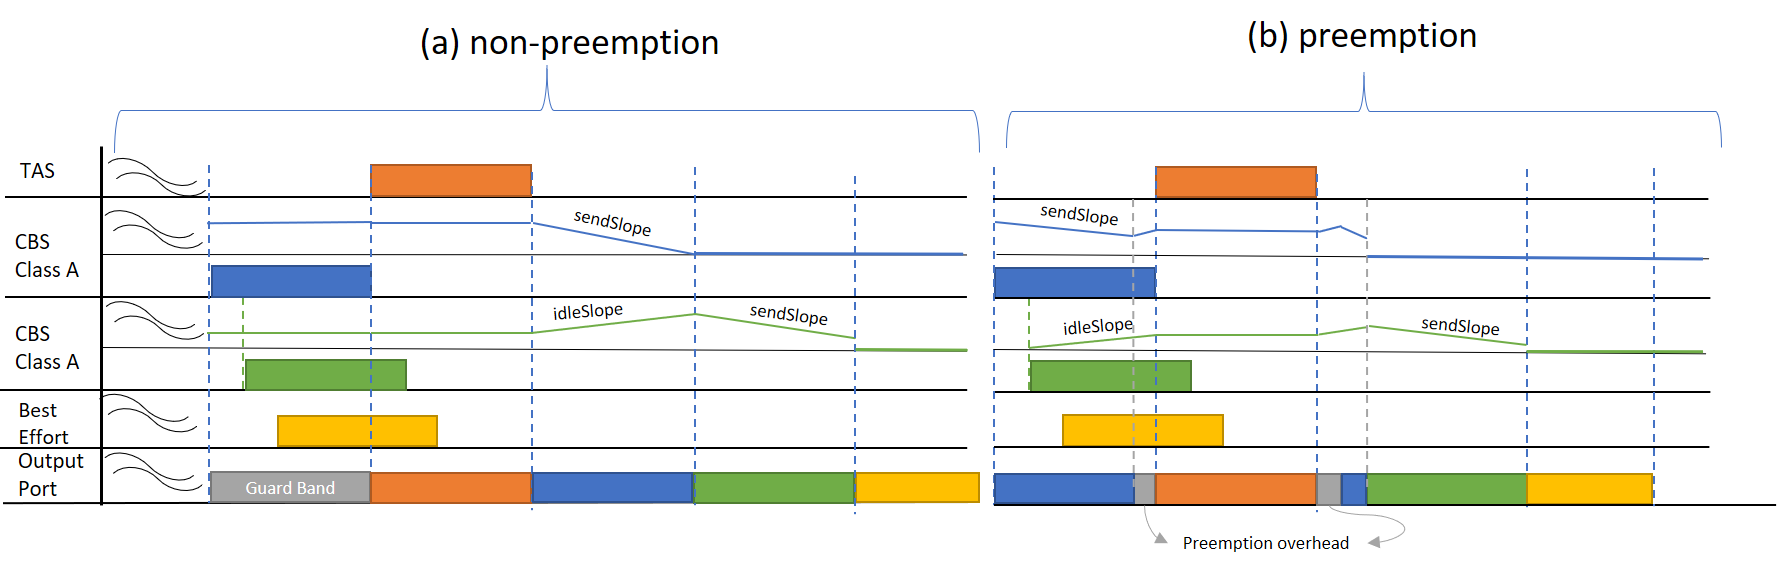
\includegraphics[width=3.5in]{TSNFlowControl}
\caption{Flow control at an output port employing TSN CBS and TAS with and without preemption}
\label{TSN_FlowControl}
\end{figure}
The flow control in general deals with the schedule of the flows in order to comply with the QoS requirements primarily latency. There are different standards that play their role in scheduling different classes of traffic in a TSN. 

IEEE 802.1Qav \cite{IEEE802.1Qav} deals with queuing and forwarding of time sensitive streams. The standard divides the time sensitive traffic in to two classes i-e Class A (tight Delay Bound) and Class B (Lose Delay Bound). It also employs Credit Based Shaper (CBS) in order to avoid starvation of Best Effort (BE) traffic that does not have delay bound. CBS is a credit-based mechanism that only allows a stream to transmit if it has non-zero, positive credit. The CBS is governed by idle slope and send slope. The CBS of a particular class is increased by idle slope if there is at least one frame (of that class) in waiting and is decreased by send slope during the transmission.

Time Aware Shaper (TAS) \cite{IEEE802.1Qbv} make use of Gate Controlled List (GCL) for a queue and it make use of global clock synchronization \cite{IEEE802.1AS}. GCLs dictate opening and closing of the gate for each queue of output port in a bridge. The gate is opened for low priority traffic if it can be closed before transmission of TAS queues. The timer period of no-activity at the gate before time critical frame is transmitted is referred to as guard band.

IEEE 802.1Qbu \cite{IEEE802.1Qbu} introduces low priority traffic frame preemption with an overhead. The guard band here gets reduced to the shortest low priority frame fragment.

\section {Analysis}
As discussed, TSN employs broad range of standards aimed at different use-cases with stringent latency requirements. In the flow control in order to schedule a packet dynamically, the scheduling entity needs to determine the schedulability of the frame i-e the latency of scheduled packet should be less than the worst case latency for the traffic. In the presence of multitude TSN standards at a node the analysis to determine the schdulability becomes involved. In this section, we review three different techniques aimed at the timing analysis primarily latency of dynamic traffic of a network.

\subsection {ML Based Analysis}
This methodology significantly differs from the other techniques discussed here as it does not explore underlying mathematical timing analysis to determine schedulability of a configuration. The paper \cite{ML} develops a machine learning model to ascertain feasibility of different configurations of a real time ethernet network as available under TSN standards. It goes on to compare performance metric, i-e accuracy and computation time, of the developed model with two network calculus based models referred to as approximate and precise in the paper.

\subsubsection{Model}
Four TSN based configurations are considered while evaluating feasible configurations for a real time ethernet network given the traffic and their associate timing constraints. The configuration are named as FIFO, Manual, Concise Priority (CP8) and Manual with traffic shaping, for details consult \cite{ML}. The configuration are proposed while keeping TSN standards in mind while consorting to the standard static priority scheduling algorithms in order to compare the ML model results with so called “approximate analysis” and “precise analysis based off  \cite{8,9,37}.

A generic topology of network is given for which three classes of traffic is scheduled namely Audio, Video and Command and Control (C\&C). The ML model that is used to determine feasibility of a configuration is K Nearest Neighbors (KNN), K being an arbitrary number of neighbors. The learning complexity of the model is O(N), N being the training data set, as it only needs to store the training data set. Each member of training data set of length N, is D dimensional, D being the number of features of a configuration having maximum impact on the end result i-e if a particular configuration having certain values of D features is feasible to schedule or not. The decision sought from the ML model is binary i-e schedulable or not schedulable.
In the training phase of the model, the labelled training data is stored in an N x D array, for instance. The decision of the feasibility against these data indices is stored in a N dimensional array where entries 0 and 1 represent non-feasibility and feasibility respectively. Once a prediction against a new configuration, i-e a D dimensional data point, is sought from the ML model, an L2 norm of the data point is calculated from the N data points stored as training data set and K closest neighbors of the data point are identified. Based on majority voting of feasibility status of K neighbors, the decision of feasible or not feasible is taken against the new configuration. Four such models are developed against the solutions proposed earlier. The computational complexity here is of order of O(NKD) for each new configuration.
In order to have accurate prediction, the training data set should be sufficient to populate D dimensional space of data points adequately. The trade off here is clear; more features of a configuration mean more apt characterization of the configuration; however, this also implies that more data points are needed to populate now higher dimensional space of the data set in order to have accurate predictions. This phenomenon is referred to as curse of dimensionality.
In the ML model developed in the \cite{ML}, following five features of a configuration are selected based on the empirical results: the number of critical flows, the number of audio flows, the number of video flows, the maximum load of the network and Gini Index. Gini Index \cite{GINI} is a quantitative characterization of unbalancedness of link loads.
\subsubsection{Results}
The training data set is generated by labelling randomly generated data of the given topology by the accurate analysis in order to avoid false negatives. The hyperparameters such as K neighbors, K fold cross validation are fine-tuned by experiments.
A training data set of N=5200 was deemed optimum against the accuracy, where any increases in N afterwards plateaued the accuracy curve.
As can be seen in Table 2 of \cite{ML} the overall accuracy reduces with increasingly complex model. True Positive Rate (TPR) captures the percentage of accurate prediction of the overall prediction deemed to be feasible by the model. The TNR is just the converse of TPR. The lower percentage of TPR in the case of FIFO is correlated by Kappa Index and F Index. The reason behind that is low coverage of D dimensional space for the case of feasible solutions. As most of the training data set contained not feasible solutions indicated by F index for the case of FIFO scheduling.
The figure 6 in \cite{ML} shows the comparison of the performance of ML model against the “approximate” and “accurate” analysis in the case of Manual Scheduling, the accuracy of the model is slightly worse than the two other two analysis. However, there is a significant difference of computation time only for the case 10\^6 TSN configurations.
The table 3 of \cite{ML} summarizes the accuracy result and make a comparison against the other two analyses. The interesting point to note is that the analyses do not yield False Positive Rate as opposed to the ML model, which might indicate potential room of improvement in the Approx. analysis as it is pessimistic. For the case of CP8 there is an improvement of overall accuracy in the case of ML model
\subsubsection{Conclusion}
The paper was premised around infeasibility of computational time in the case of accurate analysis however the choice of ML model is not consistent with the premise, since the prediction time of the model will increase linearly with the training data set.
 Another potential improvement could be feature selection, there is no evidence of different features selection for different schedulability in the paper, as can be seen in table that the accuracy has degraded with more complicated solution. Perhaps different features selection for each solution would customize the characterization of a configuration with respect to that solution and may drive the overall accuracy higher.

Furthermore, it does not provide a worst-case estimate on the latencies which remains a major draw back even for a relatively accurate model. As it does not guarantee a worst-case latency, hence it is best suitable as a verification method for the timing constraints.

\subsection {Network Calculus Based Analysis}
Network calculus is a toolset that is used in deterministic networking to compute bound on queuing, delays, buffers etc. In this paper \cite{NC} Network Calculus is used to derive an upper bound on the latency of AVB flow of TSN, which can then be used to ascertain shcedulability of the traffic.
\subsubsection {Network Calculus Background}
\begin{figure}
\centering
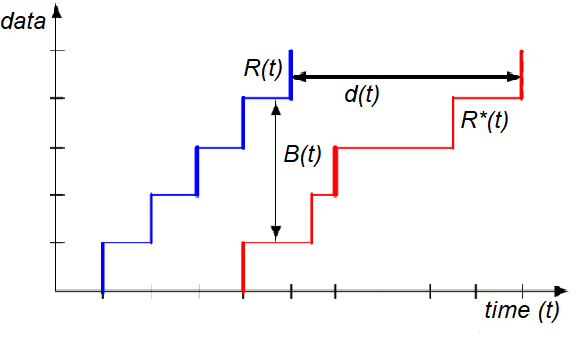
\includegraphics[width=3.5in]{NC_Background}
\caption{Arrival and Departure Functions at an arbitrary node}
\label{NC_Background}
\end{figure}
In network calculus, a system is characterized by two important functions that are arrival function $R(t)$ and departure function $R^*(t)$ as shown in the figure \ref{NC_Background}. The arrival function $R(t)$ is bounded by an arrival curve $\alpha$, which essentially is a limit on the incoming flow of the data. Similarly departure function $R^*(t)$ is bounded by a service curve $\beta$. The backlog $B(t)$ is simply a subtraction of arrival function $R(t)$ and departure function$ R^*(t)$  at a given point in time. The latency is bounded by maximum horizontal deviation between the graphs of arrival function and departure function as shown in the figure \ref{NC_Background}

The paper primarily derives expressions for arrival and service curve in order to derive a bound on arrival and departure function which then can be used to compute latency of a particular 
flow.
\subsubsection {Model}
The worst case analysis for an AVB traffic flow in presence of TT traffic is carried out by calculating the arrival and service curves of the flow. As TT traffic takes priority over any AVB flow, the paper ingeniously makes use of the arrival curves of TT traffic in order to compute service curve of the AVB flow. This makes sense because when a node is not engaged in TT traffic and credit of the particular flow is positive only then the traffic of that flow is scheduled at an output port.
\begin{figure}
\centering
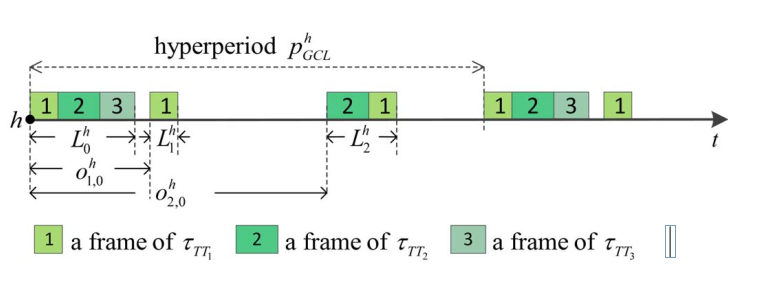
\includegraphics[width=3.5in]{NC_TT}
\caption{An example of scheduled TT traffic at an output port h }
\label{NC_TT}
\end{figure}
Since TT traffic is scheduled offline assuming in a periodic fashion as show in figure \ref{NC_TT}, this period is referred to as hyperperiod, the arrival curve for TT traffic of a particular port $h$ would simply be the summation of the bits transferred in each TT traffic window in a hyperperiod. The equation below summarizes the intuition:
\begin{equation}
\label{ttalpha}
\alpha^h_{TT,i}(i)=\sum_{j=i}^{i+N^h-1} L_j^h.C.\Bigg \lceil \frac{t-o_{j,i}^h}{\rho_{GCL}^h}\Bigg \rceil
\end{equation}
The equation represents an aggregate of arrival curves where each arrival curve is with reference to each TT traffic window.

In the case of absence of IEEE  802.1Qbu, i-e no preemption of the low priority frames, the guard period needs to be catered to in the arrival curve. For the worst case the length of guard band would be either the maximum transmission time of AVB frames or just idle period if that is shorter than the aforementioned time period. Each guard band is appended in front of each TT traffic window. Following the same logic as before, the guards bands can be nicely assimilated in to the equation by extending and adjusting the time windows of TT traffic by their corresponding guard bands as captured in the equation of arrival curve for GB and TT given by as follows:
\begingroup\makeatletter\def\f@size{8}\check@mathfonts
$$\alpha^h_{GB + TT,i}(i)=\sum_{j=i}^{i+N^h-1} (L_j^h+L_{GB,j}^h).C.\Bigg \lceil \frac{t-o_{j,i}^h+L_{GB,j}^h-L_{GB,i}^h}{\rho_{GCL}^h}\Bigg \rceil$$\endgroup

Now, considering an AVB flow of class $M$, an interval $\Delta t$ at an output port $h$ can be broken down as: $\Delta t =\Delta t^+ + \Delta t^- + \Delta t^0$ where $\Delta t^+$ refers to the time spent in waiting, $\Delta t^-$ is the time duration of the transmission and $\Delta t^0$ refers to the time duration of TT and GB windows. As service curve is a bound on the departure function, it can be well characterized by bits served in $\Delta t^-$. This knowledge along with arrival curves of the TT and GB windows help derive the service curve for the AVB flow of class M.

The arrival curves of the AVB flow are derived by the characteristics of the traffic associated with that flow  and is expressed as summation of the bursts, $\sigma$, associated with class $M$ in an output port $h$ and their long-term rate of arrival, $\rho$, expressed as: 
\begin{equation}
\label{avbalpha}
\alpha^h_{AVB\_M}(t)=\sum_{\uptau_{AVB\_M_k\in h}}\sigma_{AVB\_M_k}^h+ \sum_{\uptau_{AVB\_M_k\in h}} \rho_{AVB\_M_k}^h.t
\end{equation}
As discussed earlier, the maximum horizontal deviation of arrival and service curve of an output port $h$ draws an upper bound on the latency, $D_{AVB\_M_k,i}^h$. The arrival curve of subsequent nodes can be estimated by summing the arrival curve of the current node with upper bound of latency, D, for that node. Since service curve is dependent on reference TT windows, $i$, this yield multiple upper bounds for the latency of the flow $\uptau_{AVB\_M_k}$, the worst-case upper bound is the maximum latency, $ \max_{i} D_{AVB\_M_k,i}^h$ for the output port $h$.
\subsubsection{Results}
The paper has incorporated the analysis on a topology of 31 End Switches (ES), 15 SWs and 39 routers connected by dataflow links transmitting at 1 Gbps. In order to show the scalability of the analysis, the Worst Case Delays (WCD) of 34 AVB flows are compared against 15 and 100 TT flows. For each AVB flow the WCD in presence of 100 TT flows was greater than that of 15 TT flow, which makes sense since the service curve of AVB flow reduces with an increased value of arrival curve of TT and GB.

Similarly, the analysis goes on to show that WCD in the case of non-premption of AVB flows are always greated than premption mode due to the penalty incurred by GB. The analysis also noted that the WCD of AVB flow reduce with an increased value of idle slope. However, the degree of decrease in WCD reduces at a certain point yielding diminished returns. The analysis also explore the effect of the routing path in a TSN topology and discovers significant impact of routing on the WCD of AVB flows.
\subsubsection{Conclusion}
The paper derives expression for WCD of AVB flows in the presence of TT traffic by empoying NC toolset. The analysis captures the behaviour of a TSN traffic in a node and results shown are consistent with that behaviour. The analysis presented in the paper is comprehensive as it incorporates TT traffic along with premption and non-premption mode. The analysis claims to remove the pessismism of the results obtained in \cite{NCCOMPARE}. 

\subsection {Compositional Performance Analysis (CPA) of AVB Ethernet Traffic}
This technique \cite{CPA} differs from the NC one primarily because of the mathematical approach towards tackling the timing analysis of the network traffic. This paper makes use of CPA toolset to derive an upper bound on the latency of a traffic stream of class AVB.
\subsubsection{CPA Background}
CPA model is composed of a set of tasks that are then processed by the a set of resources. For example an output port is a resource that executes tranmission of different flows in a network that are reqarded as tasks. Each task, $\uptau_i$,  is activated by their respective events, $q$, which are frames of a particular stream that keep the task busy referred to as busy time $B(q)$, part of the busy time is the execution time of the task on the resource associated with the task. Each task has a profile of events referred to as maximum and mimimum arrival curves, these arrival curves provide the information regarding the arrival of the events associated with the task in a given time interval.
\subsubsection{CPA based Analysis}
Busy time activated by q event is given by the equation:

\begin{align*}
\label{Busytime}
B_i^+(q,a_i^q)\leq t_{transfer}(q)+I_{LPB}+I_{SPB}(a_i^q)+\\
			I_{TSB}(a_i^q)+I_{HPB}(B_i^+(q,a_i^q))
\end{align*}

where: $t_{transfer}(q) = q.C_i^+$ is maximum tranfer time for back to back q events and $C$ is the time it takes for a frame to transmit at an output port. $I_{LPB}=\max\limits_{j\in lp(i)} C_j^+$ is worst-case time taken by a lower priority task that just started execution before arrival of the q-event. $I_{SPB}(a_i^q)=\sum\limits_{j\in sp(i)} (\upeta_j^+(a_i^q).C_j^+)$ is worst-case time taken by same priority events of task $\uptau_j$ arrived until arrival time of q-event of $\uptau_i$ given by $a_i^q$. $I_{HPB}(B_i^+(q,a_i^q))=\sum\limits_{j\in hp(i)} (\eta_j^+(B_i^+(q,a_i^q)-C_i^+).C_j^+)$ is worst-case time taken by a high priority task, $\uptau_j$, following the same logic as same priority task however the subtraction of $C_i^+$ is due to the non-premption nature of onging low priority task, $I_{TSB}$ is worst-case time taken by traffic shaper or insufficient credit which is dependent on other terms of the expression as blocking of $\uptau_i$ due to any reason would result in an increase of the credit. For details consult \cite{CPA}
The upper bound on latency, $l_{p}^+$, of stream $p$ is given by the summation of the worst-case response time, $R_i^+$, at each node along the path. The derived equation is as follows:
\begin{equation*}
l_p^+ \leq \delta^-_{first(p)}(s) + \sum_{j \in Tasks(p)} R_j^++ O_{routing}(p)
\end{equation*}
where $ \delta^-_{first(p)}(s)$ is the worst-case arrival interval between the last and the first frame and $O_{routing}$ is the path delay associated between the nodes. In order to compute worst-case response time, $R_i^+$, at each node one has to find the worst-case time interval between the foremost q event arrival and the last q event departure of the same busy time characterized by $R_i^+=\max\limits_{q\in Q_i}\big\{ \max\limits_{a_i^q\in A_i}\{B_i^+(q,a_i^q)-a_i^q\}\big\}$. Different values of arrival times $a_i^q$ of qth event have to be considered which in return affect the busy time, leading to fixed point iterations.

So far in the analysis, the effect of traffic shaper has not been incorporated into the calculation of arrival times of the events, incorporating such could reduce interference of same priority tasks vying for the same resource. For that, an upper bound on the traffic shaped by a shaper on a resource is computed which is then incorporated in to the output event model for each task. For detailed derivation consult \cite{CPA}.
\subsubsection {Results}
Having developed the model for AVB traffic, the paper goes on to evaluate the model on different topologies by comparing the worst-case latencies of AVB traffic with that of strict priority. A general trend of much higer latencies in the case of AVB are observed which is explainable due to the maximum transmission bound imposed by shaper credit. It was seen that setting the idle slope of AVB traffic 31 times than the required bandwidth achieves the same latency as of strict priority. It was noted that in the case of linear topology the rate of increase of latencies with respect to the number of nodes was much higher than that observed in star topology. This is due to the intermediate shapers at each node that accumulated the effect of shaper at the output node.
\subsubsection {Conclusion}
The paper makes use of CPA analysis to compose a model of AVB ethernet traffic and evaluates the result in different topologies. The model is shown to be scalable with the plausible results. 

However, with respect to TSN standards the analysis leaves much to be desired as it does not: 1) incorporate premption of low priority frames as standarized in IEEE 802.1Qbu, 2) explicitly include effect of TT traffic on to the credit shaper.

\section {Conlcusion}
We have reviewed TSN standards particularly associated with the flow control. We then discussed three different approaches aimed at  providing the schedulability analysis of AVB traffic flow in a TSN network. We have discussed and compared the underlying mathematical principles of the aforementioned approaches. Furthermore, we also highlighted the shortcomings in the completeness of the analyses with regards to TSN standards.
%\subsection{Subsection Heading Here}
%Subsection text here.

% needed in second column of first page if using \IEEEpubid
%\IEEEpubidadjcol

%\subsubsection{Subsubsection Heading Here}
%Subsubsection text here.


% An example of a floating figure using the graphicx package.
% Note that \label must occur AFTER (or within) \caption.
% For figures, \caption should occur after the \includegraphics.
% Note that IEEEtran v1.7 and later has special internal code that
% is designed to preserve the operation of \label within \caption
% even when the captionsoff option is in effect. However, because
% of issues like this, it may be the safest practice to put all your
% \label just after \caption rather than within \caption{}.
%
% Reminder: the "draftcls" or "draftclsnofoot", not "draft", class
% option should be used if it is desired that the figures are to be
% displayed while in draft mode.
%
%\begin{figure}[!t]
%\centering
%\includegraphics[width=2.5in]{myfigure}
% where an .eps filename suffix will be assumed under latex, 
% and a .pdf suffix will be assumed for pdflatex; or what has been declared
% via \DeclareGraphicsExtensions.
%\caption{Simulation results for the network.}
%\label{fig_sim}
%\end{figure}

% Note that the IEEE typically puts floats only at the top, even when this
% results in a large percentage of a column being occupied by floats.


% An example of a double column floating figure using two subfigures.
% (The subfig.sty package must be loaded for this to work.)
% The subfigure \label commands are set within each subfloat command,
% and the \label for the overall figure must come after \caption.
% \hfil is used as a separator to get equal spacing.
% Watch out that the combined width of all the subfigures on a 
% line do not exceed the text width or a line break will occur.
%
%\begin{figure*}[!t]
%\centering
%\subfloat[Case I]{\includegraphics[width=2.5in]{box}%
%\label{fig_first_case}}
%\hfil
%\subfloat[Case II]{\includegraphics[width=2.5in]{box}%
%\label{fig_second_case}}
%\caption{Simulation results for the network.}
%\label{fig_sim}
%\end{figure*}
%
% Note that often IEEE papers with subfigures do not employ subfigure
% captions (using the optional argument to \subfloat[]), but instead will
% reference/describe all of them (a), (b), etc., within the main caption.
% Be aware that for subfig.sty to generate the (a), (b), etc., subfigure
% labels, the optional argument to \subfloat must be present. If a
% subcaption is not desired, just leave its contents blank,
% e.g., \subfloat[].


% An example of a floating table. Note that, for IEEE style tables, the
% \caption command should come BEFORE the table and, given that table
% captions serve much like titles, are usually capitalized except for words
% such as a, an, and, as, at, but, by, for, in, nor, of, on, or, the, to
% and up, which are usually not capitalized unless they are the first or
% last word of the caption. Table text will default to \footnotesize as
% the IEEE normally uses this smaller font for tables.
% The \label must come after \caption as always.
%
%\begin{table}[!t]
%% increase table row spacing, adjust to taste
%\renewcommand{\arraystretch}{1.3}
% if using array.sty, it might be a good idea to tweak the value of
% \extrarowheight as needed to properly center the text within the cells
%\caption{An Example of a Table}
%\label{table_example}
%\centering
%% Some packages, such as MDW tools, offer better commands for making tables
%% than the plain LaTeX2e tabular which is used here.
%\begin{tabular}{|c||c|}
%\hline
%One & Two\\
%\hline
%Three & Four\\
%\hline
%\end{tabular}
%\end{table}


% Note that the IEEE does not put floats in the very first column
% - or typically anywhere on the first page for that matter. Also,
% in-text middle ("here") positioning is typically not used, but it
% is allowed and encouraged for Computer Society conferences (but
% not Computer Society journals). Most IEEE journals/conferences use
% top floats exclusively. 
% Note that, LaTeX2e, unlike IEEE journals/conferences, places
% footnotes above bottom floats. This can be corrected via the
% \fnbelowfloat command of the stfloats package.




%\section{Conclusion}
%The conclusion goes here.





% if have a single appendix:
%\appendix[Proof of the Zonklar Equations]
% or
%\appendix  % for no appendix heading
% do not use \section anymore after \appendix, only \section*
% is possibly needed

% use appendices with more than one appendix
% then use \section to start each appendix
% you must declare a \section before using any
% \subsection or using \label (\appendices by itself
% starts a section numbered zero.)
%


%\appendices
%\section{Proof of the First Zonklar Equation}
%Appendix one text goes here.

% you can choose not to have a title for an appendix
% if you want by leaving the argument blank
%\section{}
%Appendix two text goes here.


% use section* for acknowledgment
%\section*{Acknowledgment}


%The authors would like to thank...


% Can use something like this to put references on a page
% by themselves when using endfloat and the captionsoff option.
\ifCLASSOPTIONcaptionsoff
  \newpage
\fi



% trigger a \newpage just before the given reference
% number - used to balance the columns on the last page
% adjust value as needed - may need to be readjusted if
% the document is modified later
%\IEEEtriggeratref{8}
% The "triggered" command can be changed if desired:
%\IEEEtriggercmd{\enlargethispage{-5in}}

% references section

% can use a bibliography generated by BibTeX as a .bbl file
% BibTeX documentation can be easily obtained at:
% http://mirror.ctan.org/biblio/bibtex/contrib/doc/
% The IEEEtran BibTeX style support page is at:
% http://www.michaelshell.org/tex/ieeetran/bibtex/
%\bibliographystyle{IEEEtran}
% argument is your BibTeX string definitions and bibliography database(s)
%\bibliography{IEEEabrv,../bib/paper}
%
% <OR> manually copy in the resultant .bbl file
% set second argument of \begin to the number of references
% (used to reserve space for the reference number labels box)


%\bibliographystyle{plain}

%\begin{thebibliography}{1}

%s\bibitem{IEEEhowto:kopka}
%H.~Kopka and P.~W. Daly, \emph{A Guide to \LaTeX}, 3rd~ed.\hskip 1em plus
 %0.5em minus 0.4em\relax Harlow, England: Addison-Wesley, 1999.

%\bibitem {new}
%\end{thebibliography}
\bibliographystyle{IEEEtran}
\bibliography{new}

% biography section
% 
% If you have an EPS/PDF photo (graphicx package needed) extra braces are
% needed around the contents of the optional argument to biography to prevent
% the LaTeX parser from getting confused when it sees the complicated
% \includegraphics command within an optional argument. (You could create
% your own custom macro containing the \includegraphics command to make things
% simpler here.)
%\begin{IEEEbiography}[{\includegraphics[width=1in,height=1.25in,clip,keepaspectratio]{mshell}}]{Michael Shell}
% or if you just want to reserve a space for a photo:

%\begin{IEEEbiography}{Michael Shell}
%Biography text here.
%\end{IEEEbiography}

% if you will not have a photo at all:
%\begin{IEEEbiographynophoto}{John Doe}
%Biography text here.
%\end{IEEEbiographynophoto}

% insert where needed to balance the two columns on the last page with
% biographies
%\newpage

%\begin{IEEEbiographynophoto}{Jane Doe}
%Biography text here.
%\end{IEEEbiographynophoto}

% You can push biographies down or up by placing
% a \vfill before or after them. The appropriate
% use of \vfill depends on what kind of text is
% on the last page and whether or not the columns
% are being equalized.

%\vfill

% Can be used to pull up biographies so that the bottom of the last one
% is flush with the other column.
%\enlargethispage{-5in}



% that's all folks
\end{document}


